\documentclass[conference]{IEEEtran}
\IEEEoverridecommandlockouts

\usepackage{cite}
\usepackage{amsmath,amssymb,amsfonts}
\usepackage{graphicx}
\usepackage{textcomp}
\usepackage{xcolor}
\usepackage{booktabs}
\usepackage{array}
\usepackage{algorithm}
\usepackage{algpseudocode}
\usepackage{dblfloatfix}
\usepackage{float}

\graphicspath{{images/}}

\begin{document}

\title{Using ID3 Decision Trees to Classify and Analize Data}

\author{
    \IEEEauthorblockN{Jacob A. Geldbach}
    \IEEEauthorblockA{
        \textit{College of Engineering: CS} \\
        \textit{University of Idaho} \\
        Moscow Idaho, United States \\
        geld8788@vandals.uidaho.edu
    }
}

\maketitle

\begin{abstract}
% TODO: 3-5 sentences. What did you build (ID3 decision tree, entropy/information-gain
% splitting), what dataset/decision problem (7 binary attributes -> robot asks for
% help vs. decides on its own, 100 examples), what experiment was run (sweep of
% training-set sizes, N random trials per size, measuring held-out test accuracy /
% precision / recall and tree size), and a one-line headline result (e.g. how accuracy
% and tree size trended with more training data, and whether the root attribute stayed
% stable).
   In this project, Information Theory was used in order to build an ID3 decision tree from a subset of data entries, this subset known as the training subset was picked randomly from a given set of 100 example data entries. Each entry is defined as 7 different binary attributes indicating if that attribute for that example was true or not. The outcome attribute of each entry indicates if the robot in that scenario asked for help or not or decides on its own. The remainder of data entries not included in the training subset then are used to make up the testing subset. The ID3 Decision tree built from the training subset was then tested against the testing subset where accuracy and other error measuring metrics were recorded and compared against runs of different training subset size.
\end{abstract}

\begin{IEEEkeywords}
    Decision Tree, ID3, Information Theory, Entropy, Supervised Learning, Classification
\end{IEEEkeywords}

% =======================================================
\section{Algorithm Description}
    The algorithm for this project was aimed at producing a decision tree from a subset of data so that the testing subset's error rates could be classified and compared. Specifically a Ross Quinlan 1986 ID3 greedy most information gained first implementation was used to generate a decision tree. Wherein the program will begin with a training subset size input from 1-99, wherein that many rows of data from the given 100 row dataset are randomly chosen to comprise that run or trials training subset. Once the training subset for this run has been made up, each attributes Inforamtion Gained is calculated using the Information Equation shown in Eq.~\eqref{eq:info}, which is also talked about further in the next section. The attribute with the highest calculated Information Gain is then chosen to be the root of the tree, and this is repeated until there are no non-zero attributes left from this training subset. Each row that comprises the testing subset (100 row dataset - the training subset) is then tested against this built tree, where starting at the root of the tree, the attribute is looked up in the datarow and the tree is traversed until a terminal yes or no state is seen indicating that the decision tree has decided if the robot on that run asked for help or not. The answer the tree found for that data row is recorded. Once all data rows in the training subset are ran through the decision tree, a confusion matrix for this trial is calculated by comparing the decision trees answer (predicted) vs the data rows answer (actual). This confusion matrix allows for accuracy, recall and precision to be calulcated for that trial. The program was built so that many trials at this size could be ran (all with same sized training sets but randomly made up) and the error metrics could then be averaged across the multiple runs of the same training subset size. 

\subsection*{Measuring Information}
% TODO: Explain entropy I(p1,...,pn) = -sum p_i log2(p_i) over the class distribution
% of "Decision" (Yes/No) for a set of rows, and information gain = I(parent) minus the
% size-weighted average of I(child) over the 0/1 partitions produced by splitting on a
% candidate attribute. Explain how best_attribute() picks the attribute with the
% maximum information gain at each node (the classic ID3 greedy, one-step-lookahead
% splitting rule), and why this is a greedy/local choice rather than a globally optimal
% tree search.
    The 1 bit of Information Gained or Entropy calculation shown in Eq.~\eqref{eq:info} is what the algorithm uses each iteration to choose the next attribute in the tree. Omitting any attributes that have already been chosen that run from the calculation it simply chooses which attribute this equation gives the highest value for based on the attributes and their probabilties in the comprised training subset.

\begin{equation}
    I\big(p(v_1),\dots,p(v_n)\big) \;=\; -\sum_{i} p(v_i)\,\log_2 p(v_i)
    \label{eq:info}
\end{equation}

\subsection*{Handling Undefined Cases}
% TODO: Discuss the edge cases the implementation had to special-case:
%   - p_i = 0 terms are skipped in the entropy sum (0*log2(0) is defined as 0, log2(0)
%     is undefined, so those terms are never evaluated).
%   - Empty rows subsets (a branch value that appears in 0 training rows) get
%     information() = 0 and, in build_tree, become a leaf labeled with the parent's
%     majority label (the default_label passed down the recursion) rather than
%     recursing on nothing.
%   - Pure subsets (all one class) short-circuit to a leaf immediately, no gain
%     calculation needed.
%   - Running out of attributes on a path (all 7 already used) with a still-mixed
%     class distribution: falls back to a majority-label leaf instead of splitting
%     further.
%   - Information-gain ties between candidate attributes are broken deterministically
%     by the fixed attribute order from the CSV header (first attribute in that order
%     wins), and majority-label 50/50 ties are broken by first-seen class order via
%     Counter.most_common(1) -- both choices matter for reproducibility across trials.
%   - The "full data" sweep condition (training size == all 100 rows) leaves no
%     held-out test rows; accuracy/precision/recall are left blank for that condition
%     while tree-size/depth/root-attribute are still recorded.
    There were two undefined scenarios in the inforamtion calculating and building of the tree that needed to be addressed. The first was when an attribute has p_i = 0. This will lead to Eq.~\eqref{eq:info} being undefined as \log_2(0) goes to -INF, not to mention the attribute has a probibilty of 0 so it is simply skipped and not considered in the built decision tree. The 2nd case being when two attributes produce valid but equal gain. The tie breaker used in this implementation was simply which attribute came first in the CSV ordering, and this was kept consistent across all runs since the CSV was structured the same throughout.

\subsection*{Measuring Performance}
% TODO: Explain the experiment design used to measure performance:
%   - Sweep over training-set sizes N (e.g. 10..90), for each size draw `trials`
%     independent random train/test splits (train_test_split(), without replacement,
%     remaining rows held out as the test set).
%   - Per trial: build a tree with build_tree() on the training rows, then score it on
%     the held-out test rows using confusion-matrix counts (tp/fn/fp/tn with "Yes" =
%     ask-for-help as the positive class), from which accuracy, precision, and recall
%     are derived. Explain why recall (catching cases where the robot should have
%     asked for help) is the more safety-relevant metric here versus plain accuracy.
%   - Also record tree_size (node count) and tree_depth per trial, to see whether
%     larger training sets produce larger/smaller/same-sized trees, and whether the
%     root_attribute stays stable across random subsets of a given size.
%   - Aggregate across trials per size: mean and standard deviation of each metric.
%   - NOTE (write this up yourself below): the results table shows train_accuracy /
%     train_precision / train_recall = 1.000 at every training size. Explain why: with
%     no pruning, build_tree() keeps splitting until every leaf is pure (or attributes
%     run out), and this dataset has zero attribute patterns with conflicting labels,
%     so the training set is always perfectly fit -- it's a sanity-check/baseline
%     column, not a bug, and it sets up the train/test gap (overfitting) story.


% =======================================================
\section{Results}

% Figure 1 -- accuracy error (1 - accuracy), train vs. test curve, vs. training set
% size. Generated by analyze.py -> results/accuracy_error_vs_size.png.
\begin{figure}[H]
\centering
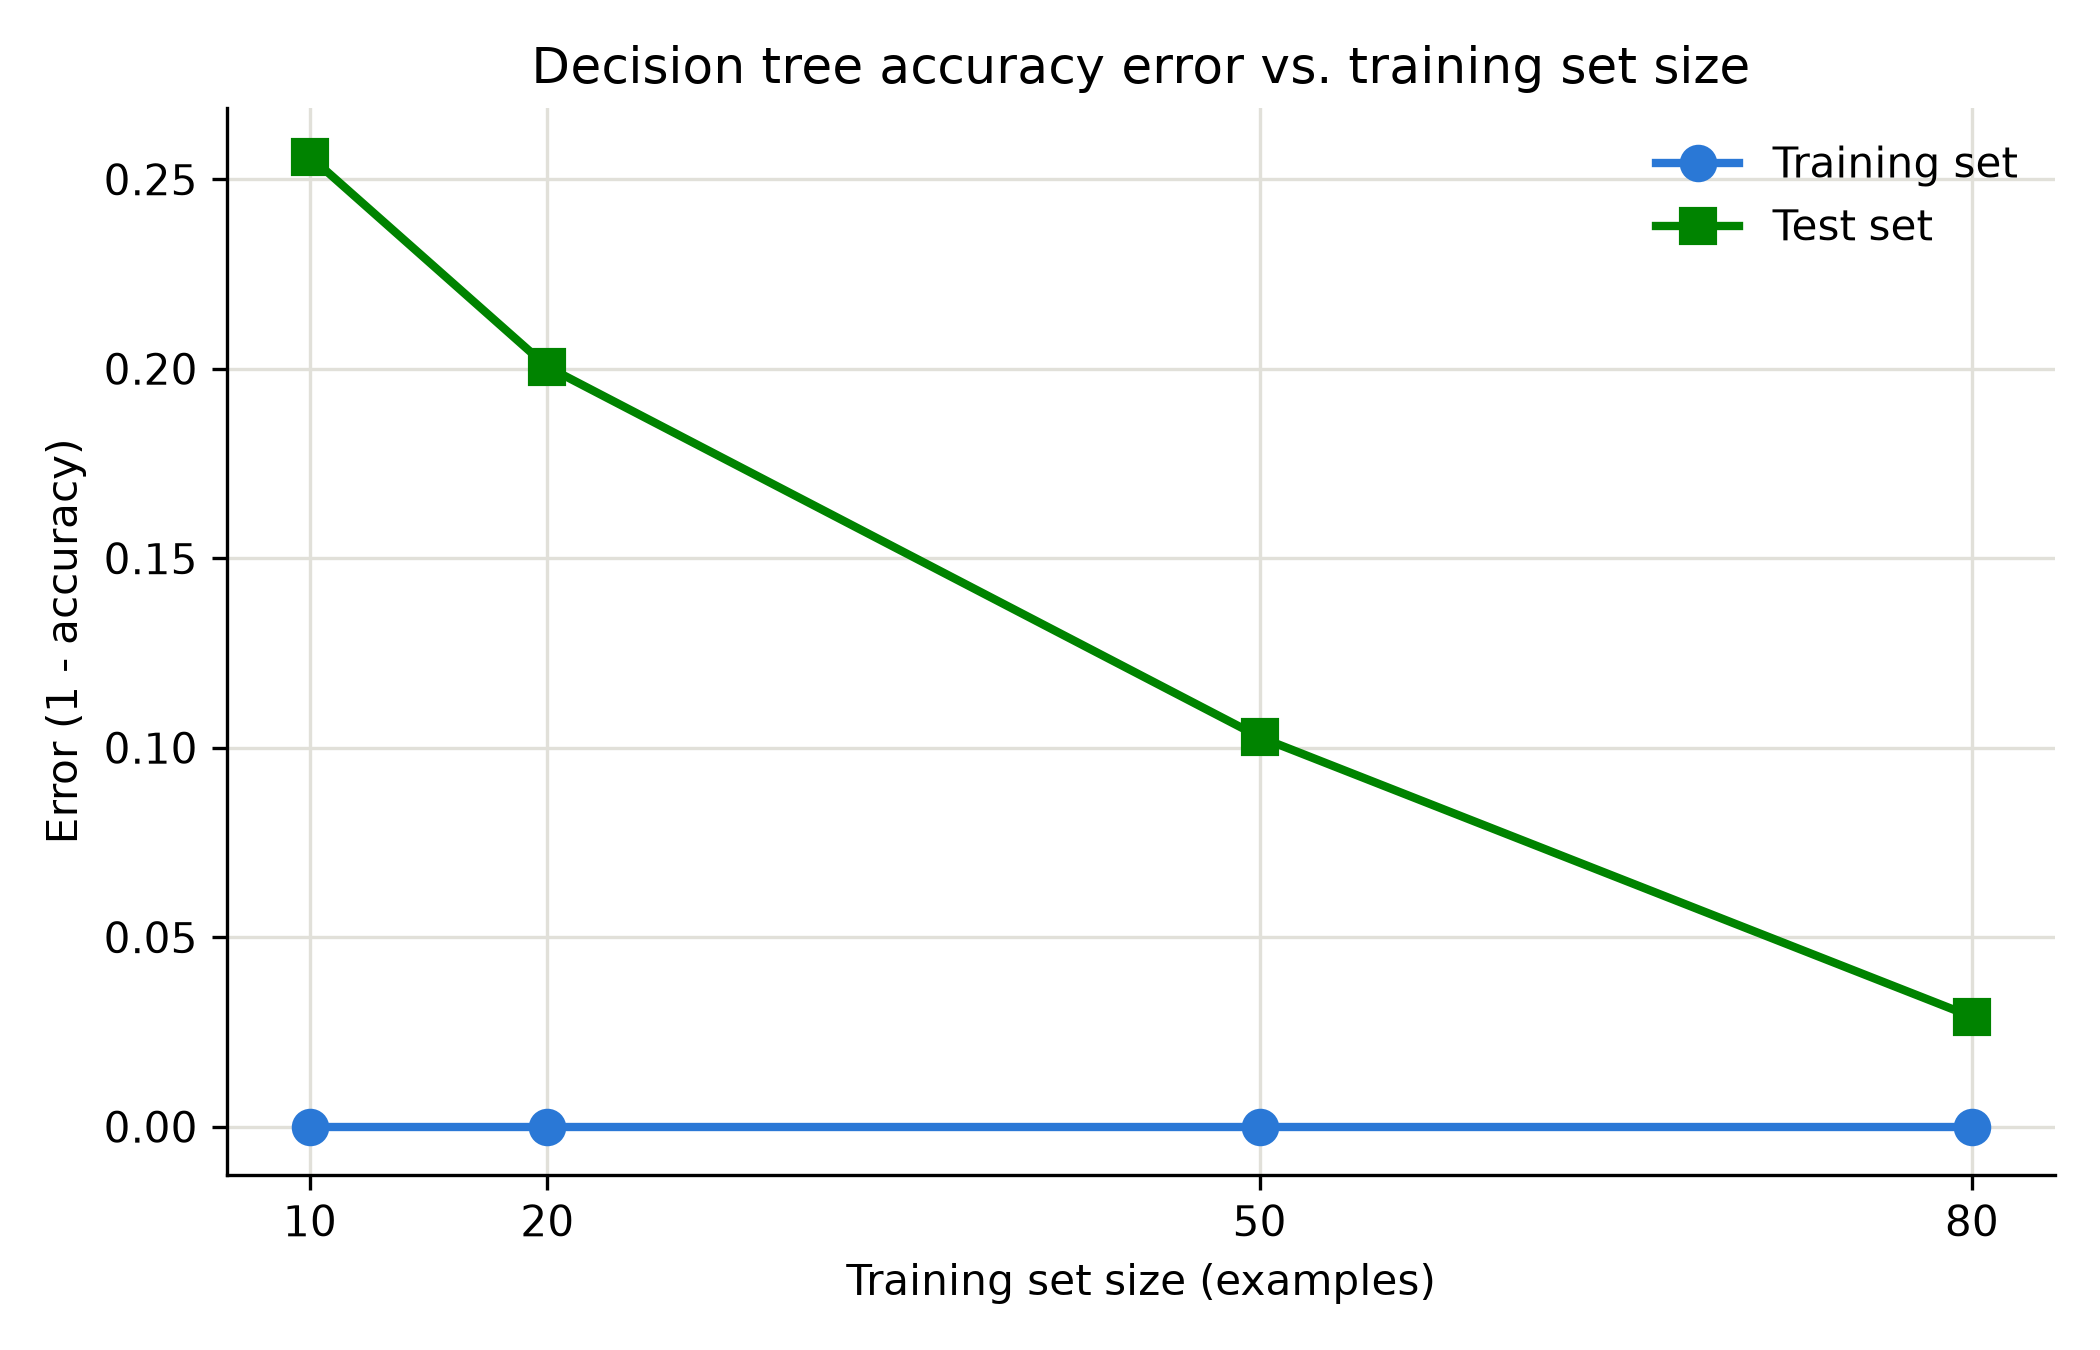
\includegraphics[width=\linewidth]{accuracy_error_vs_size}
\caption{ Accuracy error ($1 - $accuracy) vs. training set size, training-set curve
          vs. held-out test-set curve (mean over 50 trials per size).
        }
\label{fig:accuracy_error_vs_size}
\end{figure}

% Figure 2 -- recall error (1 - recall), train vs. test curve, vs. training set size.
% Recall (catching cases where the robot should have asked for help) is the more
% safety-relevant metric here. Generated by analyze.py -> recall_error_vs_size.png.
\begin{figure}[H]
\centering
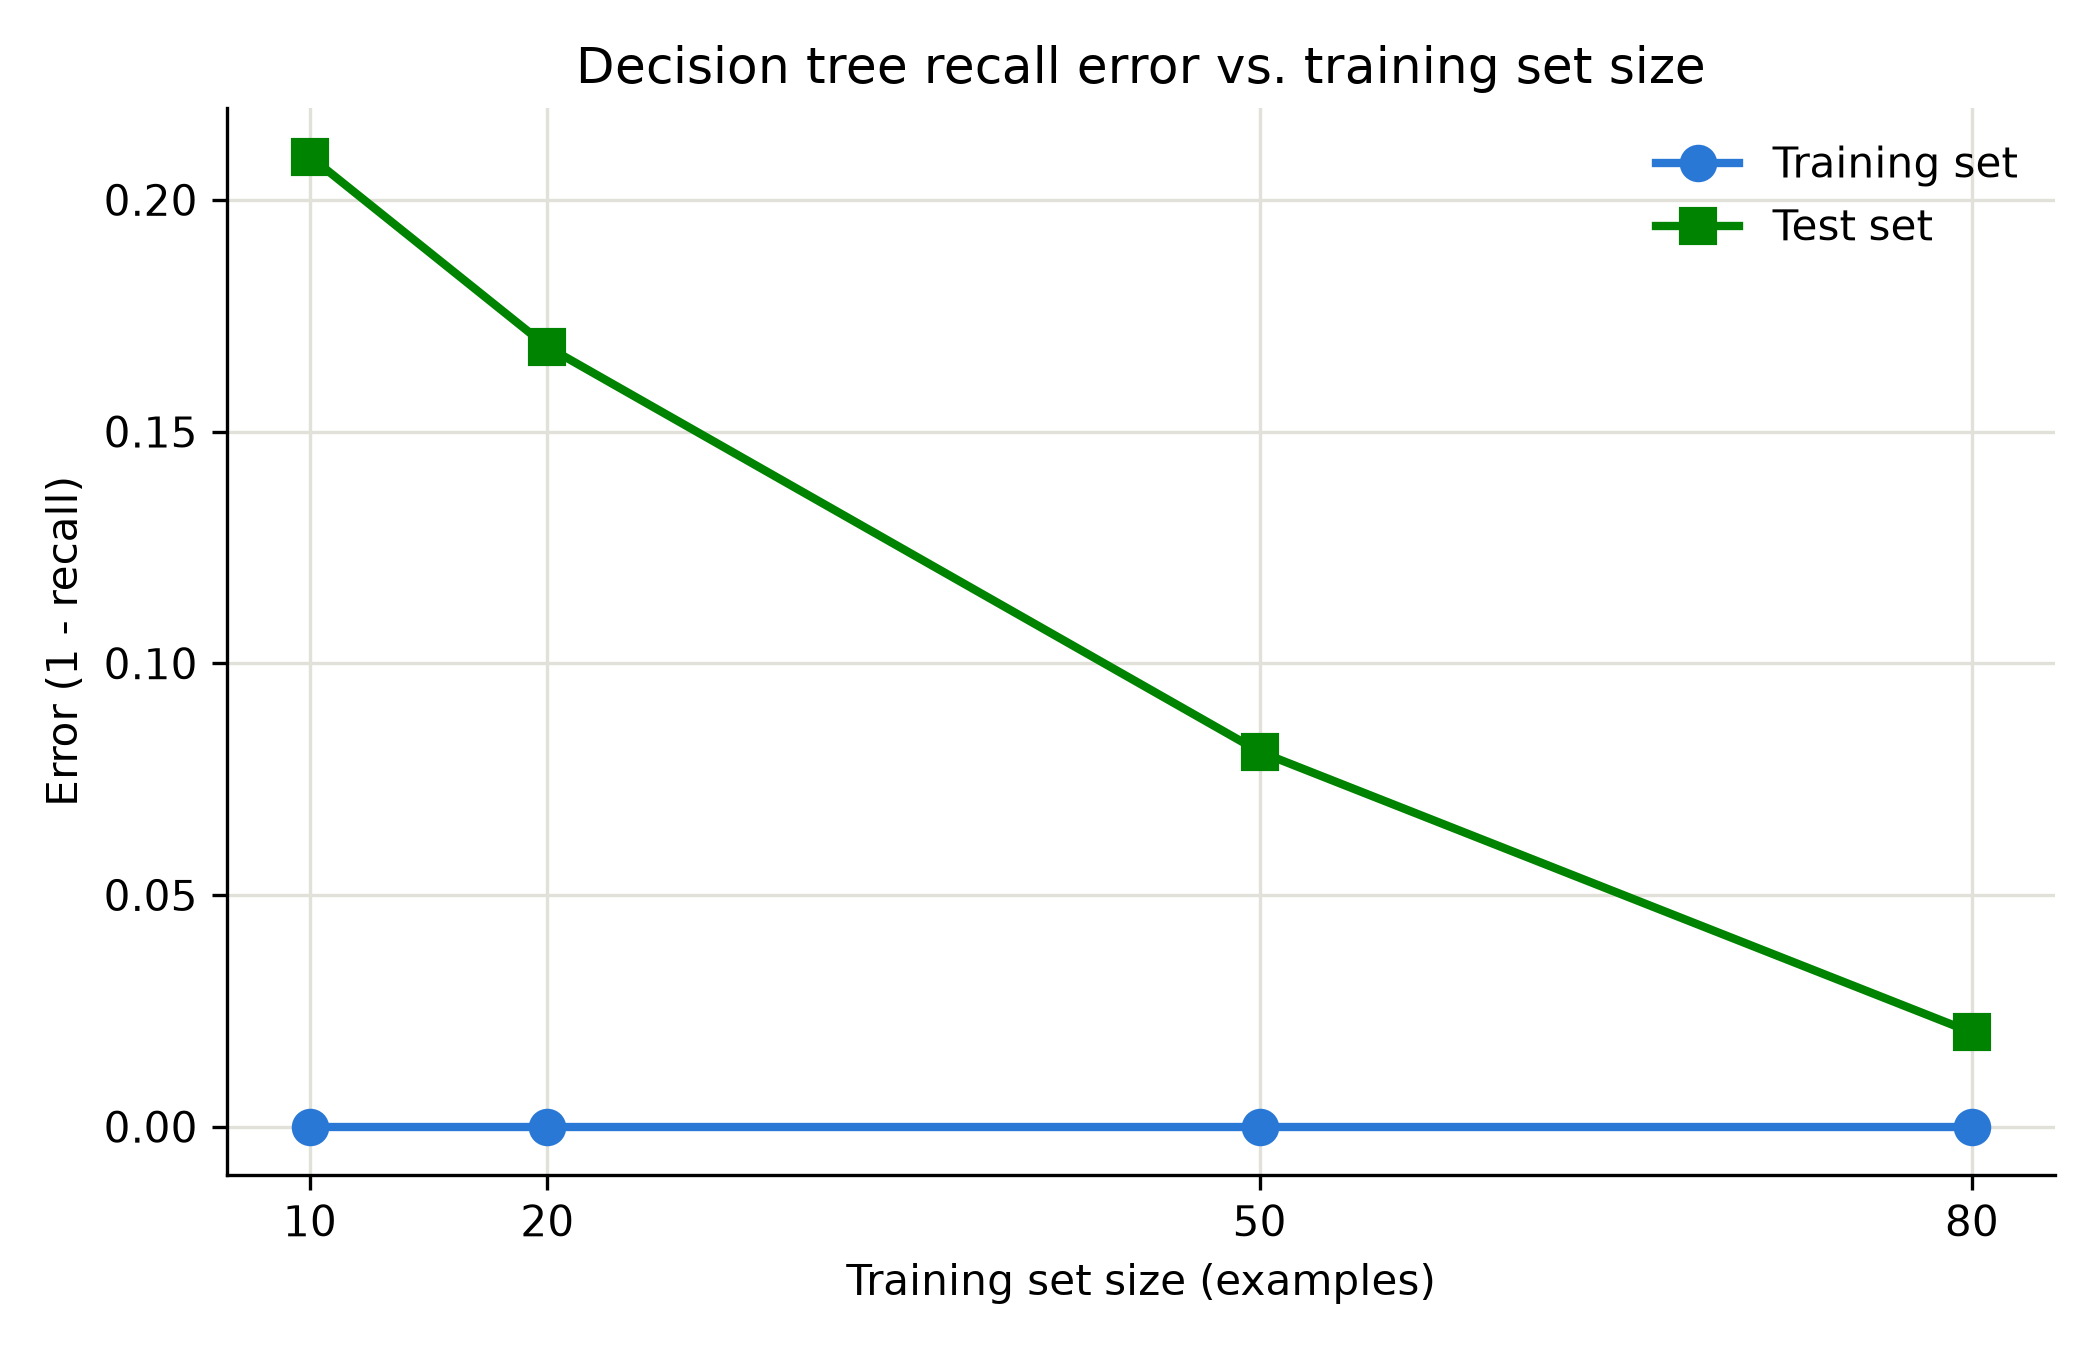
\includegraphics[width=\linewidth]{recall_error_vs_size}
\caption{ Recall error ($1 - $recall) vs. training set size, training-set curve vs.
          held-out test-set curve (mean over 50 trials per size).
        }
\label{fig:recall_error_vs_size}
\end{figure}

% TODO (optional): precision_error_vs_size.png is also in images/ if you want a third
% error figure -- 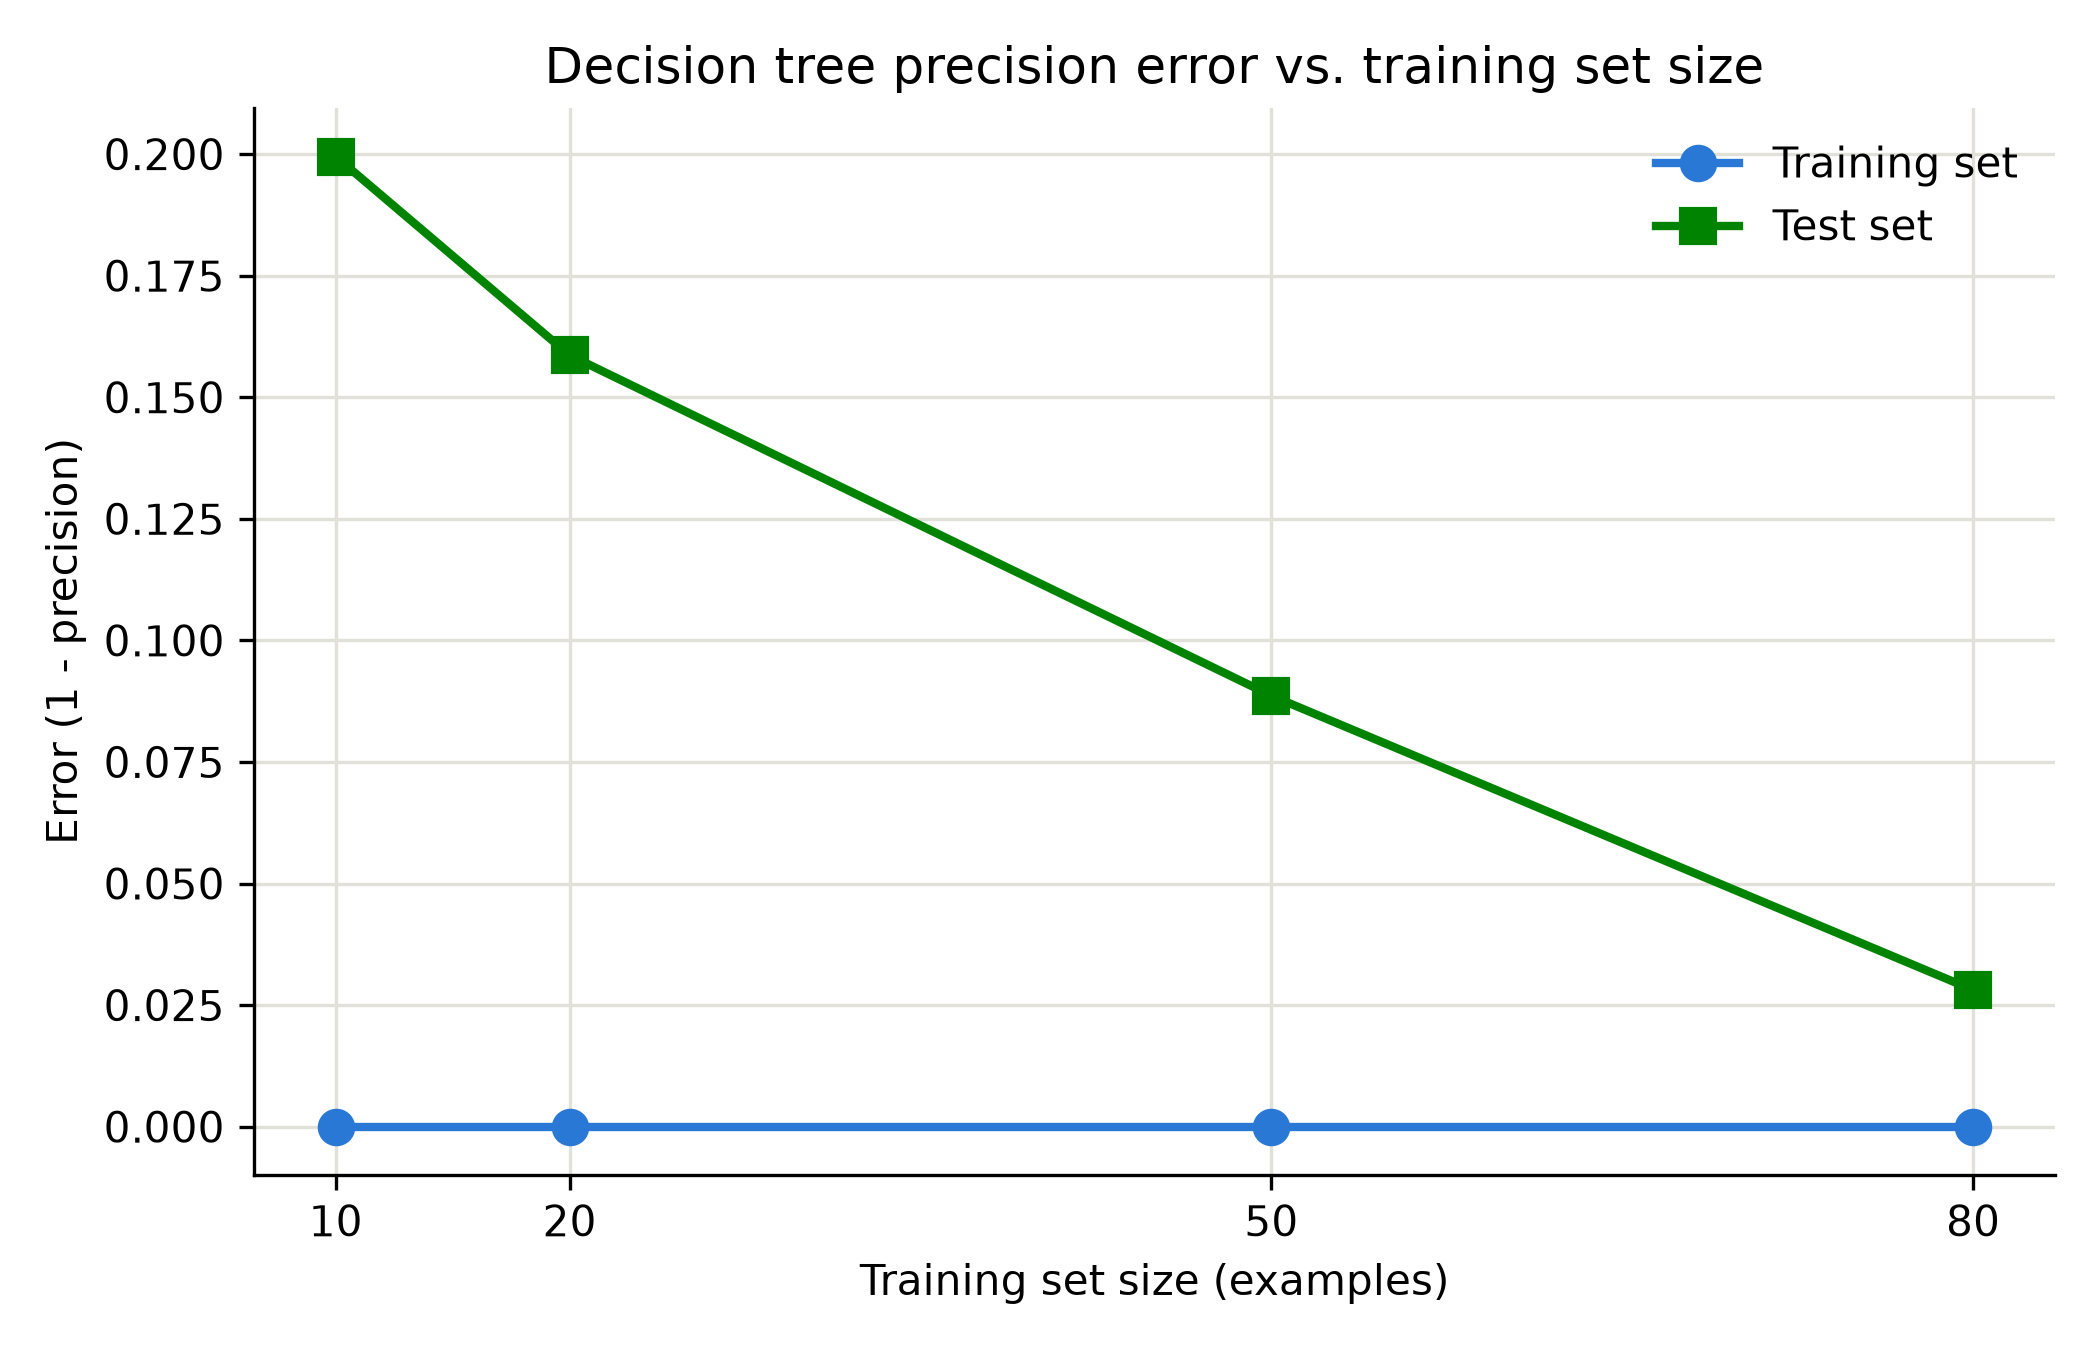
\includegraphics[width=\linewidth]{precision_error_vs_size}

% Figure 3 -- tree size (node count) vs. training set size.
% Generated by analyze.py -> results/tree_size_vs_size.png.
\begin{figure}[H]
\centering
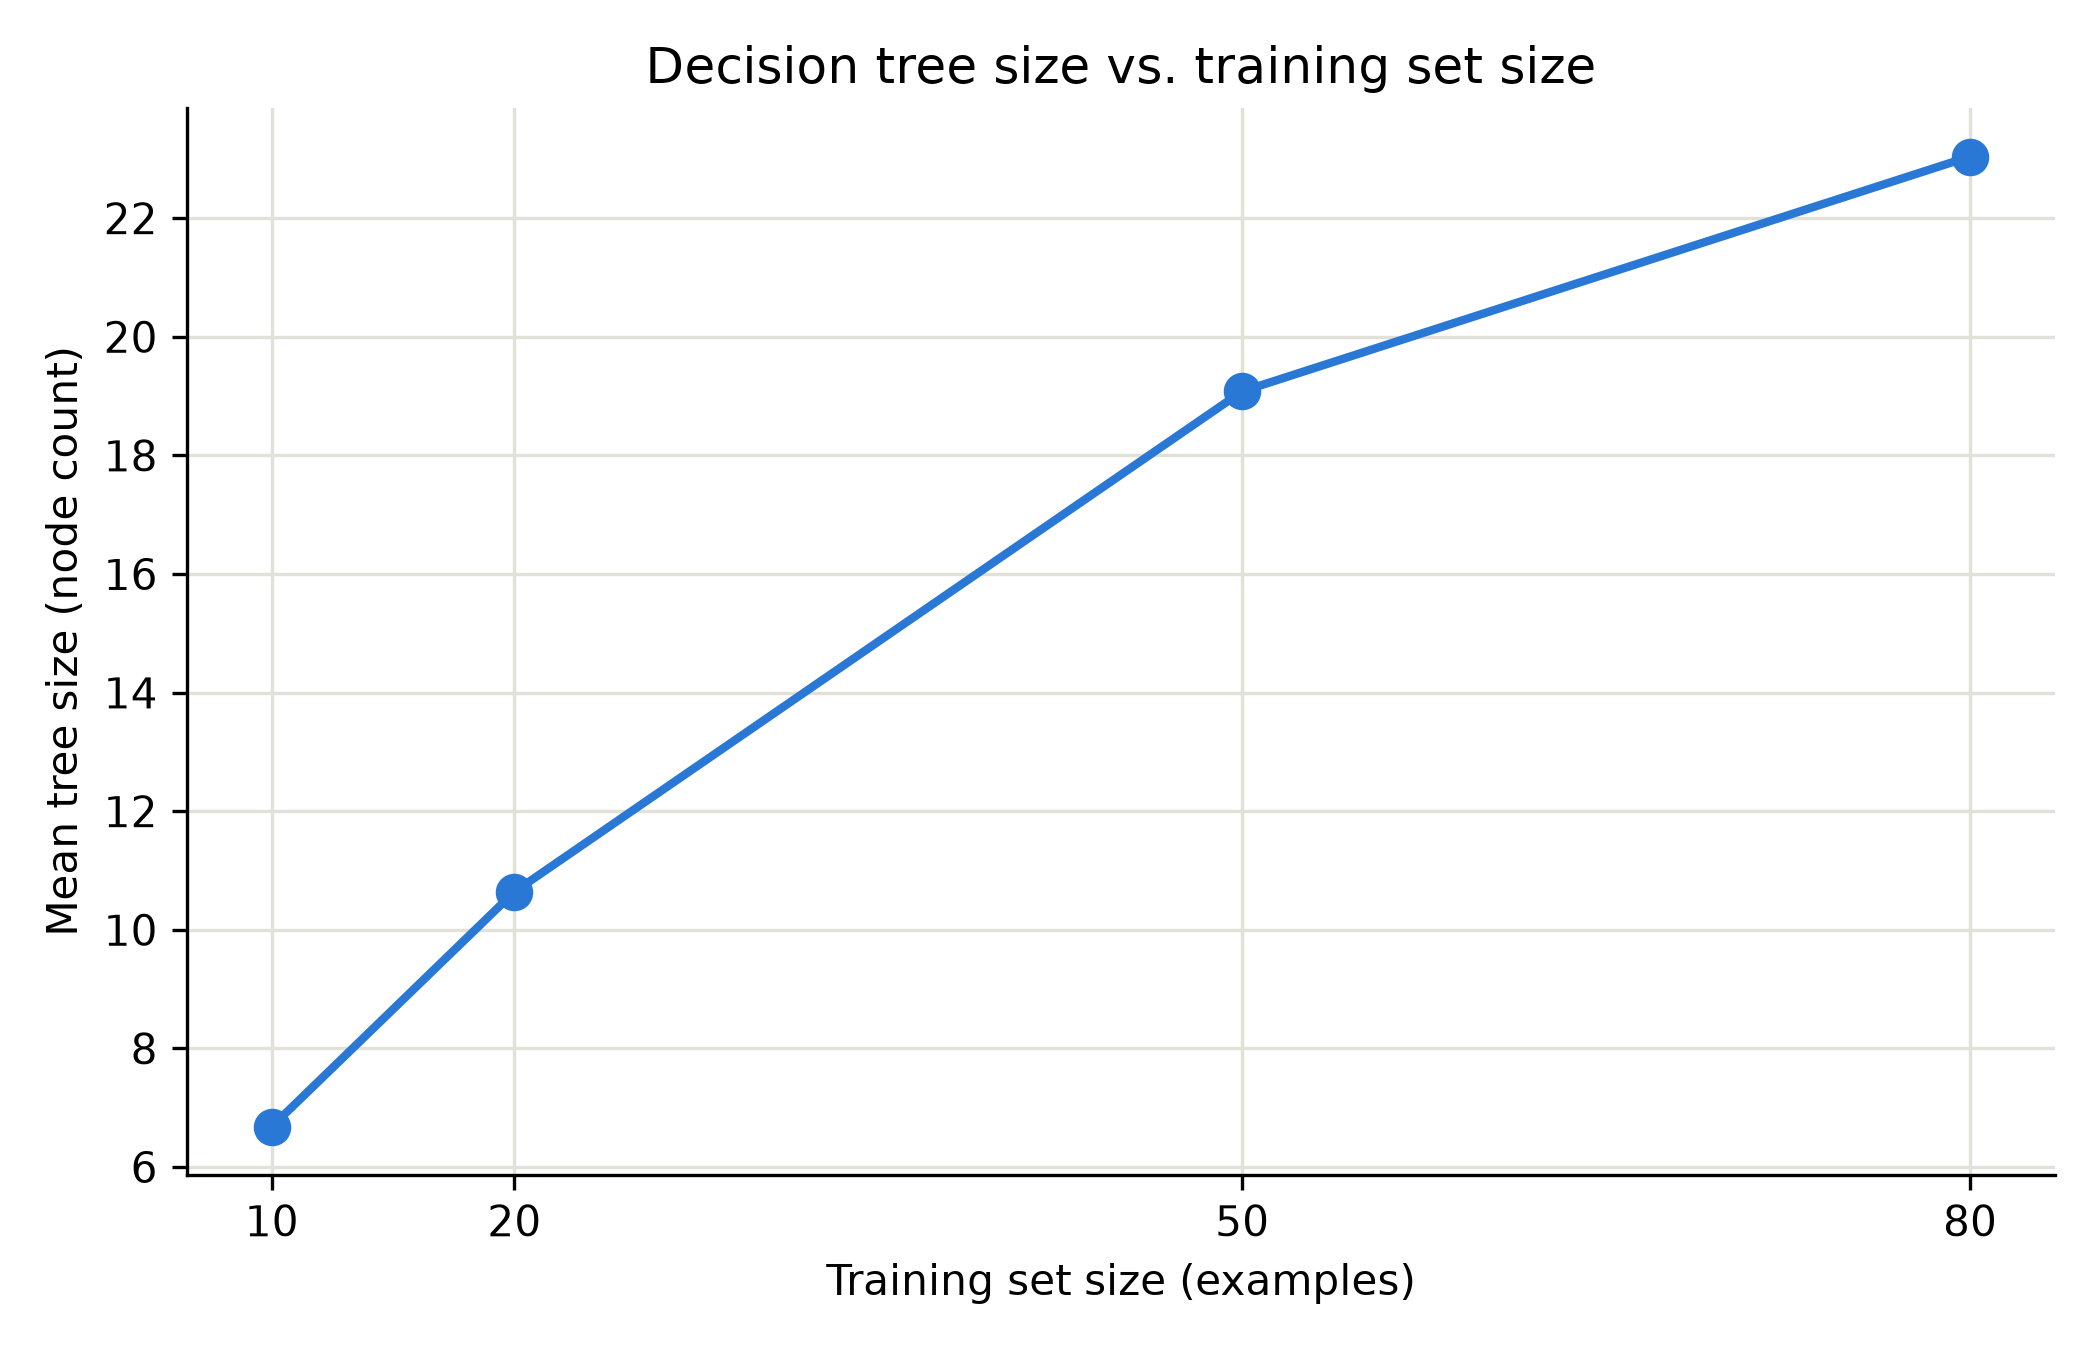
\includegraphics[width=\linewidth]{tree_size_vs_size}
\caption{ Mean decision tree size (node count) vs. training set size
          (mean over 50 trials per size).
        }
\label{fig:tree_size_vs_size}
\end{figure}

% -------------------------------------------------------
% Data from results/summary.csv (4 sizes x 50 trials each, seed = size value).
\begin{table*}[t]
\caption{ID3 Decision Tree --- Sweep Results (50 trials per training-set size)}
\begin{center}
\footnotesize
\setlength{\tabcolsep}{6pt}
\begin{tabular}{c c c c c c c c c c}
\toprule
\textbf{Train Size} & \textbf{Trials} & \textbf{Train Acc.} & \textbf{Test Acc.} & \textbf{Test Prec.} & \textbf{Test Recall} & \textbf{Mean Tree Size} & \textbf{Mean Tree Depth} & \textbf{Most Common Root Attr.} \\
\midrule
10 & 50 & 1.000 & 0.744 & 0.800 & 0.791 & 6.68  & 2.62 & Safe Situation \\
20 & 50 & 1.000 & 0.800 & 0.841 & 0.832 & 10.64 & 3.62 & Safe Situation \\
50 & 50 & 1.000 & 0.897 & 0.911 & 0.919 & 19.08 & 4.90 & Safe Situation \\
80 & 50 & 1.000 & 0.971 & 0.972 & 0.980 & 23.04 & 5.08 & Safe Situation \\
\bottomrule
\end{tabular}
\label{tab:results}
\end{center}
\end{table*}

% TODO (optional): if you visualize a specific built tree (visualization.py), include
% a screenshot here as a figure, similar to the before/after map figure in Project 3.

% =======================================================
\section{Discussion / Conclusions}
% TODO: Synthesize the table and graphs using specific numbers. Address:
%   - How did test accuracy trend with training set size? Did it plateau, and if so
%     around what size / accuracy value?
%   - How did tree size (and depth) trend with training set size -- did larger
%     training sets produce larger, smaller, or similarly-sized trees? Why, in terms
%     of ID3's greedy splitting and how many distinct attribute-value patterns show
%     up as training data grows?
%   - Did the root attribute stay stable across random subsets of a given size, or did
%     it vary trial to trial? What does that say about how much information that
%     attribute carries relative to the others?
%   - Any small-training-size pathologies (e.g. very small or very large trees,
%     unstable/high-variance accuracy) worth calling out?
%   - NOTE (write this up yourself): tie the constant 1.000 train_accuracy/precision/
%     recall column back to the shrinking train/test gap as size grows (size 10 gap
%     ~0.26 down to size 80 gap ~0.03) -- that shrinking gap is the overfitting story,
%     the training column itself is expected to be flat, not evidence of a problem.

\subsection*{Strengths and Weaknesses}
% TODO: Strengths -- e.g. ID3 is simple, fast, fully deterministic given a fixed
% training set, produces an interpretable/human-readable tree, no hyperparameters to
% tune. Weaknesses -- e.g. greedy one-step-lookahead splitting can miss globally
% better trees, no pruning so it can overfit on small/noisy training sets, ties broken
% arbitrarily by attribute/label order which is a bit unprincipled, only supports
% binary attributes/labels, high variance in accuracy at very small training sizes
% due to which 10 (or however few) examples happened to be sampled.
    Placeholder text on strengths and weaknesses.

\subsection*{Future Improvements}
% TODO: e.g. add pruning (reduced-error or cost-complexity) to fight overfitting,
% k-fold cross-validation instead of a single random split per trial for lower-variance
% estimates, extend to non-binary/continuous attributes, add a confidence measure at
% leaves (e.g. class proportion) instead of a hard majority label, ensemble methods
% (bagging/random forest) to reduce variance, more training examples collected overall.
    Placeholder text on possible improvements.

% =======================================================
\section*{Use of AI}

\subsection*{Coding}
% TODO: Which tool(s)/model(s), and how used (initial code, debugging, APIs, tests,
% other). Be specific about which files/tasks AI helped with vs. what you wrote by hand.
    Placeholder text describing AI use in coding.

\subsection*{Writeup}
% TODO: Whether AI helped draft/revise the write-up, how, and how you ensured the
% final text reflects your own understanding. (Write N/A if you used none.)
    Placeholder text describing AI use in the writeup.

\end{document}
